\chapter{Introduction}
In satellite applications, radio communication is usually the only way of communications between a spacecraft and the control systems here on Earth. This means that all the commands issued by the operator and the telemetry and experiment data we can gather has to go through the radio link. Also, the satellite housekeeping data, important for the estimation of the satellites' health are required to be download to the operator via a radio link. For many missions, lack of radio communication with satellite causes the mission to fail, as there is no possibility to download experiment data, even if they can be carried out automatically.

\section{Satellite radio communication}
The goal of the satellite radio communication is to establish a radio link between the satellite and the ground station. The link is usually two-directional - to receive the data from the satellite (such as telemetry - information about the current status of the satellite) and telecommands (commands issued to the satellite), but the one-way link also exists - for example, for only measuring some parameters or for periodic experiments. The two ways of a link are called uplink and downlink (fig. \ref{intro:uplink_downlink}). 
\begin{figure}[h]
    \centering
    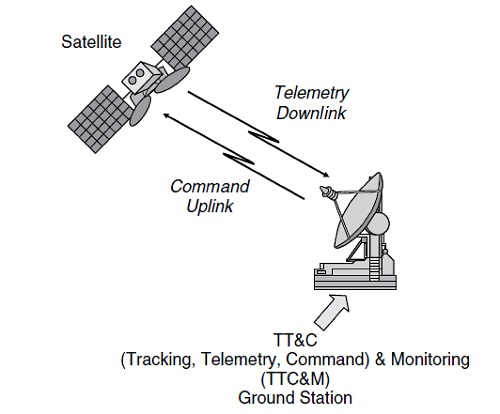
\includegraphics[width=0.5\paperwidth]{img/2/uplink_downlink.jpg}
    \caption{Satellite link uplink and downlink. Source: \cite{satcom_decription}}
    \label{intro:uplink_downlink}
\end{figure}

Depending on the altitude of the orbit (fig. \ref{intro:orbits}), the distance between the satellite and the ground station varies - from Low Earth Orbit, with altitudes \SI{200}{\kilo\meter}~-~\SI{2000}{\kilo\meter}, via Geostationary Equatorial Orbit (\SI{35786}{\kilo\meter}) up to deep space communication ($2\cdot 10^{9}$~km for Voyager 1). Different types of orbit present different difficulties - and completely different solutions are deployed on small CubeSats than large geostationary communication satellites. Depending on the orbit, the satellite can be visible only for short periods of time (as on LEO) or can be constantly monitored by the ground station (GEO). The main challenges the satellite link present are the large distance between the nodes, propagation and loss due to the atmosphere, but also limited resources on the satellite. The link consists of two nodes - the satellite and the ground station, with much different characteristics and design required. The satellite has limited dimensions and power available for the transmitter, the available space technology and power limit different antenna pointing possibilities and the available processing power. On the other hand, the ground station can be built as large as needed, with high-gain antennas, power amplifier and high-sensitivity receivers to complement the limitations of the satellite. This characterises the link as highly asymmetrical, with very high losses between the nodes and high processing gain on the ground station.
\begin{figure}
    \centering
    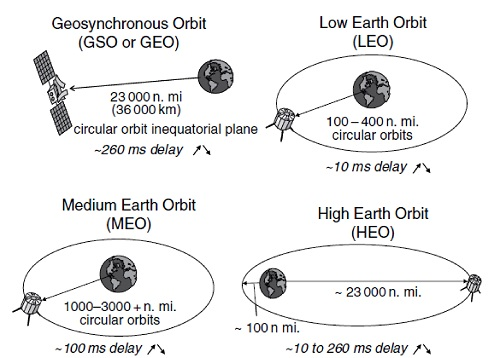
\includegraphics[width=0.4\paperwidth]{img/2/orbit_types.jpg}
    \caption{Different orbits and distances. Source: \cite{satcom_decription}}
    \label{intro:orbits}
\end{figure}

\section{Scope of the thesis}
The aim of this thesis was to design, verify, validate and deploy the communication system for fourth Polish satellite, PW-Sat2. The design covers all aspects of communication link design from the system point of view: the link design, space and ground segments and testing all the subsystems. The thesis should describe the choices, and the practical design of the low-cost satellite link using both off-the-shelf hardware, custom-designed components and Software Defined Radio, with custom digital signal processing. The designed system should provide a two-way data link between the operator and the satellite. Finally, the system was tested on the orbit, proving its parameters and reliability.

Since the beginning of the project on 4 January 2013, more than 100 students participated in the PW-Sat2 project. At the moment there are 26 active students in the team. In the team, I was responsible for the communication with the satellite (scope of this thesis), hardware design, and embedded software development. In my engineering thesis, I have designed the RadFET experiment, flown onboard PW-Sat2.
